\section{INTRODUCTIE}
Gravitationele lenzing is een effect dat optreedt wanneer licht afgebogen wordt door het gravitatieveld van massieve objecten, zoals sterrenstelsels of clusters. Deze objecten bevatten doorgaans veel donkere materie. \cite{informationesoorg-no-date}. De afbuiging van het licht kan zowel Newtoniaans als relativistisch afgeleid worden. De Newtoniaanse afleiding voor een hyperbolische baan is te vinden in \cref{appendix: newton}. In tegenstelling tot klassieke lenzing, waarbij één object wordt afgebeeld op één ander object, kan bij gravitationele lenzing één object afgebeeld worden op meerdere objecten \cite{unknown-author-2022}. Dit is te zien in \cref{fig:grav lens}. 
\begin{figure}
    \centering
    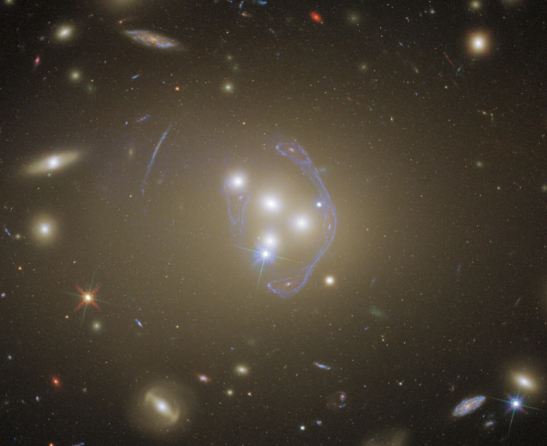
\includegraphics[width=0.95\linewidth]{Figures/gravitationele_lens.png}
    \caption{Gravitationele lens, foto van \cite{unknown-author-no-date-gravlens}}
    \label{fig:grav lens}
\end{figure}
Dit wordt bepaald door de lensvergelijking. De afleiding van de lensvergelijking in 1D is te vinden in \cref{appendix:lensvergelijking}.\\ \\
Om meer informatie te kunnen krijgen over de gravitationele lens kan het heel nuttig zijn om alle beelden die de lens genereert terug te vinden. De grotere beelden gaan voornamelijk informatie geven over de vorm van de lens, terwijl de kleinere beelden veelal informatie geven over de massaverdeling ervan. \\ \\
Soms kan het voorkomen dat een object afgebeeld wordt achter de zware massa zelf. Op \cref{fig:grav lens} zijn vijf beelden te zien. Het aantal beelden dat de lens genereert is berekend, en is gelijk aan negen. Dat wil zeggen dat er nog vier beelden zijn die niet gevonden worden doordat ze achter de lens zelf staan. Deze vier beelden geven echter wel cruciale informatie over de massaverdeling van de lens. Omdat het geweten is dat de zware massa voornamelijk uit donkere materie bestaat zou informatie over de massaverdeling ervan meer inzichten kunnen geven in donkere materie. Het doel van deze bachelorproef is het wegwerken van de zware massa op de voorgrond, om de achtergrond waar te kunnen nemen. \\ \\
Er bestaan al een heel aantal manieren waarop dit gedaan kan worden. Voorbeelden hiervan zijn IMFIT \cite{chen-2020}, \cite{erwin-2015} en GALFIT \cite{peng-2010}, \cite{unknown-author-no-date-galfit}.
In deze bachelorproef wordt er gebruik gemaakt van Bayesiaanse statistiek in de toekomst zou er ook met deep learning gewerkt kunnen worden.



